\section{Investigating Numerical stability for Fluid-Structure Interaction Problems}
The following section will give a brief insight in to the effects of choosing different $\theta$ values in the $\theta-$scheme for different time steps. 
The benchmark tests FSI2 and FSI3, as discussed in the previous section, has been investigated since they are known to be numerical unstable for certain values of $\theta$ and $\Delta t$. Only the effects of Drag as been studied as the three other quantities shows similar behavior. 
The impact of different $\theta$ values on energy stability in the solid mechanical benchmark CSM3 is also investigated.\newline

\ref{fig:FSI2drag_plots} show the plots of Drag with $\Delta t = 0.01$, showing the instability when choosing $\theta = 0.5$. The Crank-Nicholson scheme is stable until about 13 seconds where we see that it is numerically unstable and the solver diverges. While the shifted Crank-Nicholson, $\theta = 0.5 + \Delta t$, is stable throughout the computing time.\newline

\begin{figure}[H] 
  \begin{minipage}[b]{0.6\linewidth}
    \centering
    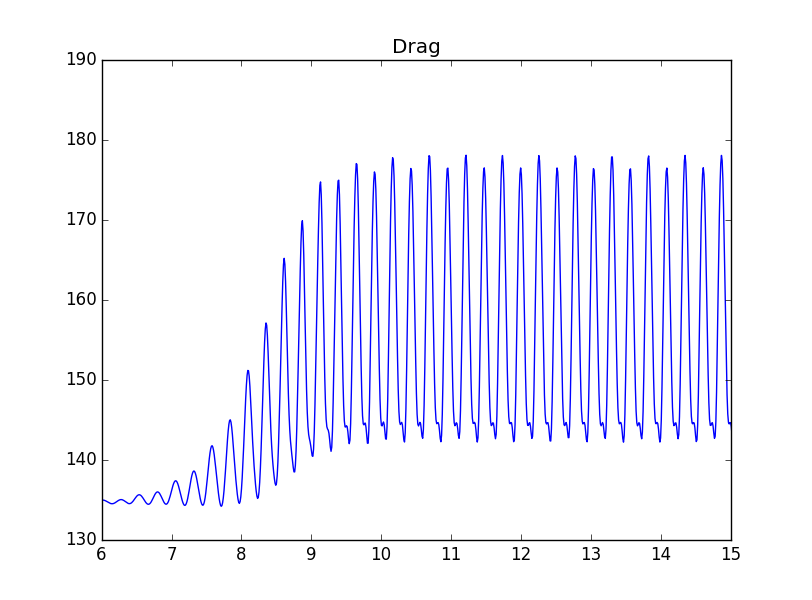
\includegraphics[scale=0.40]{./Temporal_stability/FSI2_001_051_big.png} 
    \caption{$\theta = 0.50 + \Delta t $} 
    \vspace{4ex}
  \end{minipage}%%
  \begin{minipage}[b]{0.6\linewidth}
    \centering
    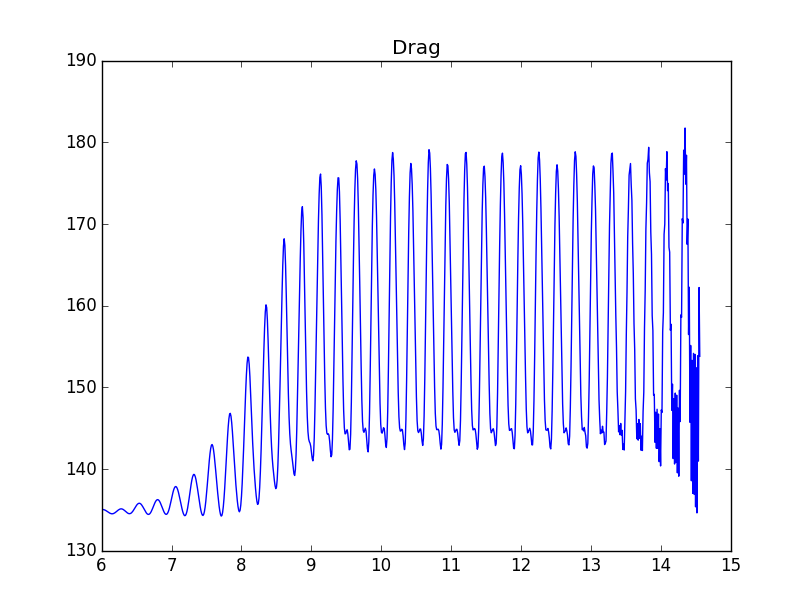
\includegraphics[scale=0.40]{./Temporal_stability/FSI2_001_050_big.png} 
    \caption{$\theta = 0.50 $} 
    \vspace{4ex}
  \end{minipage} 
  \begin{minipage}[b]{0.6\linewidth}
    \centering
    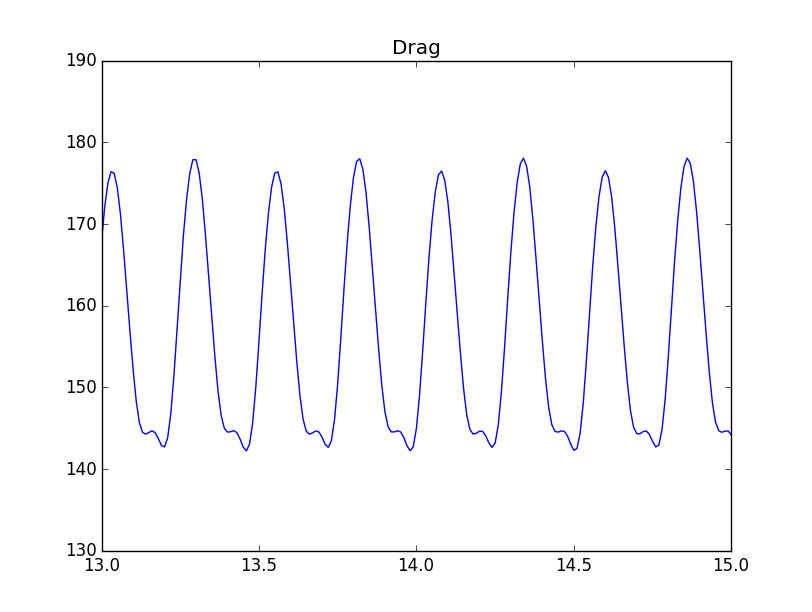
\includegraphics[scale=0.40]{./Temporal_stability/FSI2_001_051_small.png} 
    \caption{$\theta = 0.50 +\Delta t $} 
    \vspace{4ex}
  \end{minipage}%% 
  \begin{minipage}[b]{0.6\linewidth}
    \centering
    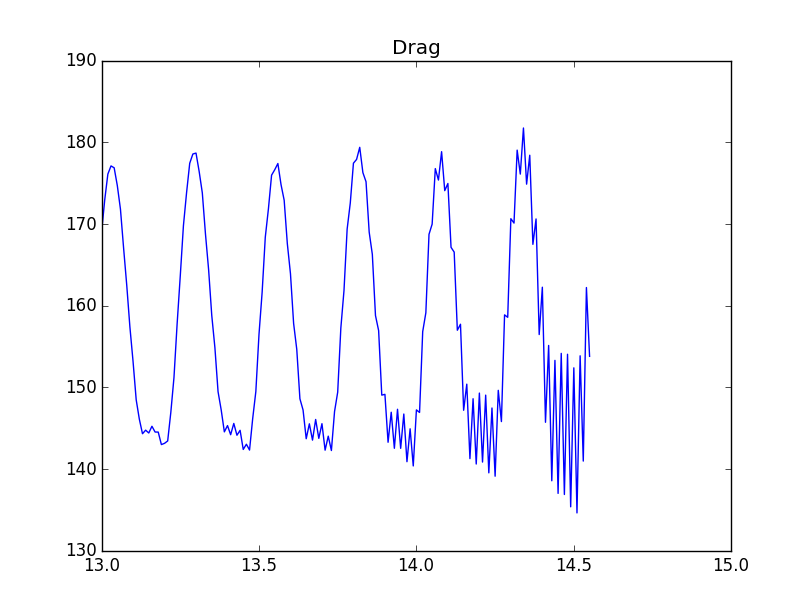
\includegraphics[scale=0.40]{./Temporal_stability/FSI2_001_050_small.png} 
    \caption{$\theta = 0.50 $} 
    \vspace{4ex}
  \end{minipage} 
\caption {Drag for FSI2 with $\Delta t = 0.01$ with different values for $\theta$}
\label{fig:FSI2drag_plots} 
\end{figure}

Figures \ref{fig: FSI3_long_short} show drag for FSI3 simulation with $\Delta t = 0.001$ and $\theta = 0.5$, showing long term stability for the normal Crank-Nicholson scheme.

\begin{figure}[H]
\begin{tabular}{ll}
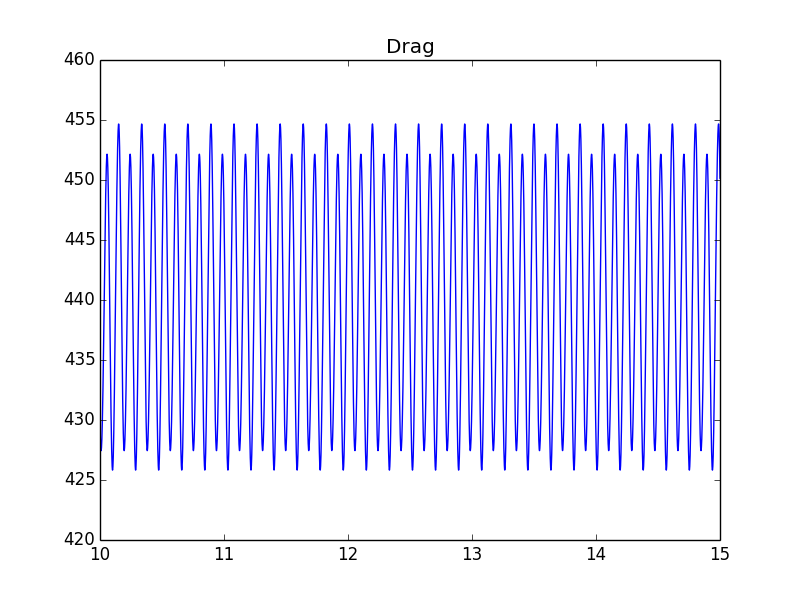
\includegraphics[scale=0.4]{./Temporal_stability/FSI3_0001_050_big.png}
&
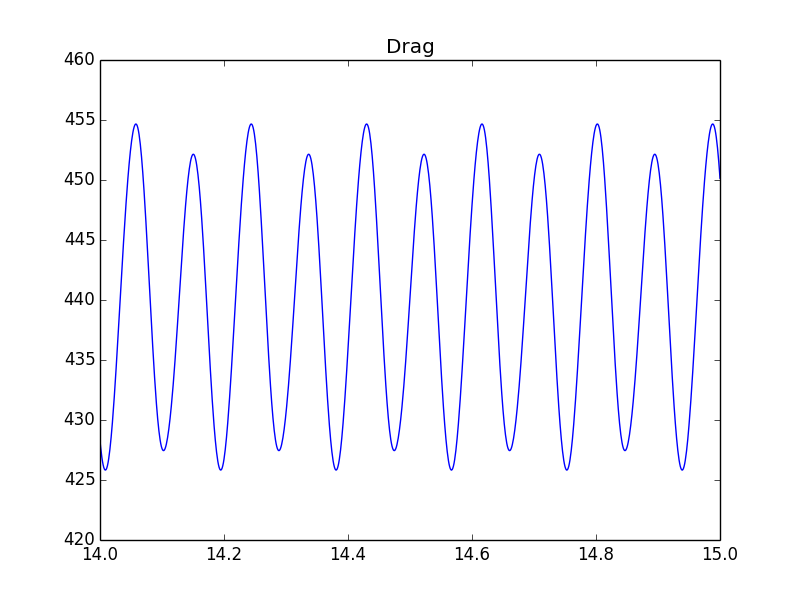
\includegraphics[scale=0.4]{./Temporal_stability/FSI3_0001_050_small.png}
\end{tabular}
\caption{FSI3 drag plot, with $\Delta t = 0.001$ and $\theta =0.5$ showing long term numerical stability}
\label{fig: FSI3_long_short}
\end{figure}

For the CSM3 case only the solid bar is computed, and with an applied force g and no friction, the bar should move down and bounce back up infinitely, for a correct solution.

Figure \ref{fig:CSM3_dis_plots} shows plots of the displacements in x and y directions for $\theta = 0.5$ and $1$. With the implicit scheme ($\theta=1$) the bar moves to a steady state solution. This means energy has not been preserved and the energy dissipates. While in the Crank-Nicholson scheme ($\theta = 0.5$), the bar moves down and back up. This indicates that the Crank-Nicholson scheme is energy preserving.

\begin{figure}[H] 
  \begin{minipage}[b]{0.6\linewidth}
    \centering
    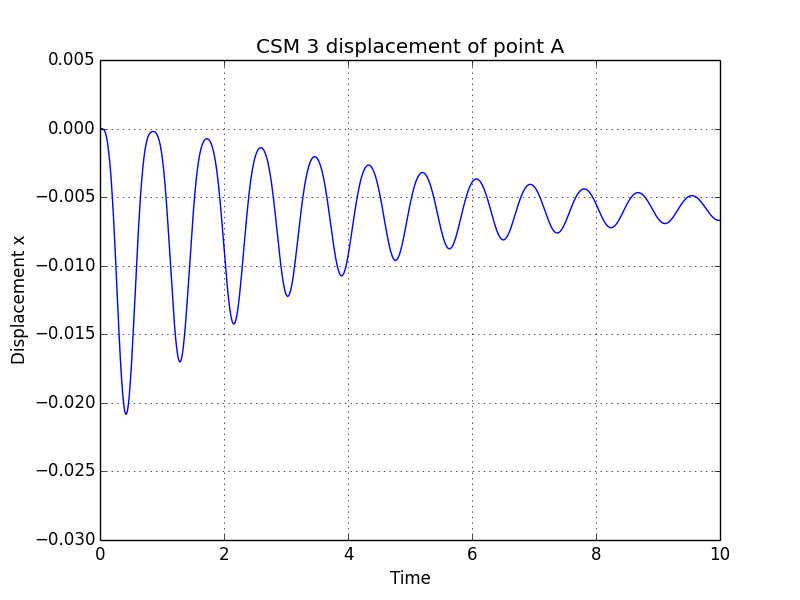
\includegraphics[scale=0.40]{./Temporal_stability/CSM3_implicit.png} 
    \caption{$\theta = 1 $} 
    \vspace{4ex}
  \end{minipage}%%
  \begin{minipage}[b]{0.6\linewidth}
    \centering
    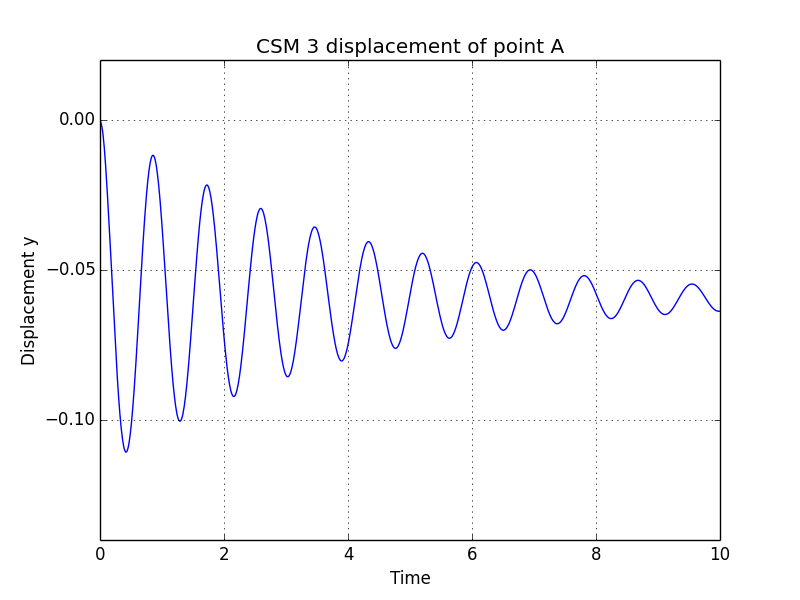
\includegraphics[scale=0.40]{./Temporal_stability/CSM3_implicit_y.png} 
    \caption{$\theta = 1 $} 
    \vspace{4ex}
  \end{minipage} 
  \begin{minipage}[b]{0.6\linewidth}
    \centering
    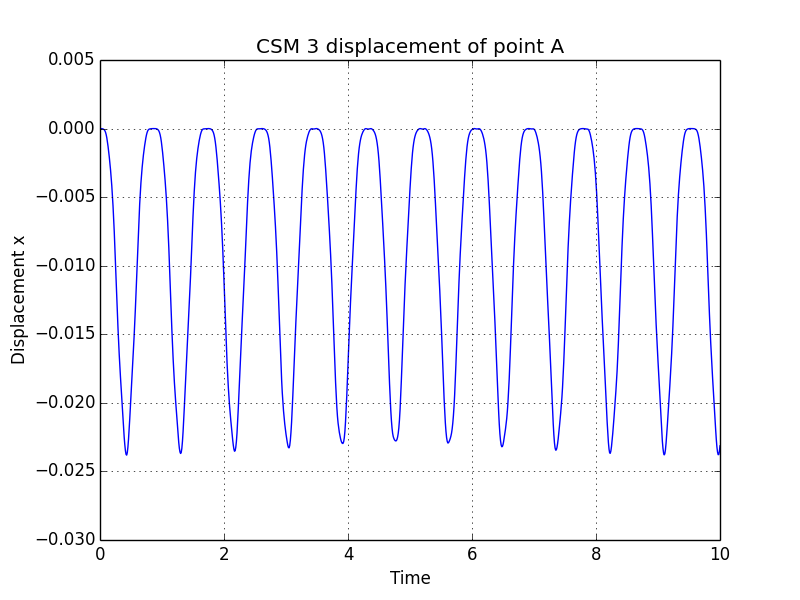
\includegraphics[scale=0.40]{./Temporal_stability/CSM3_Crank.png} 
    \caption{$\theta = 0.5 $} 
    \vspace{4ex}
  \end{minipage}%% 
  \begin{minipage}[b]{0.6\linewidth}
    \centering
    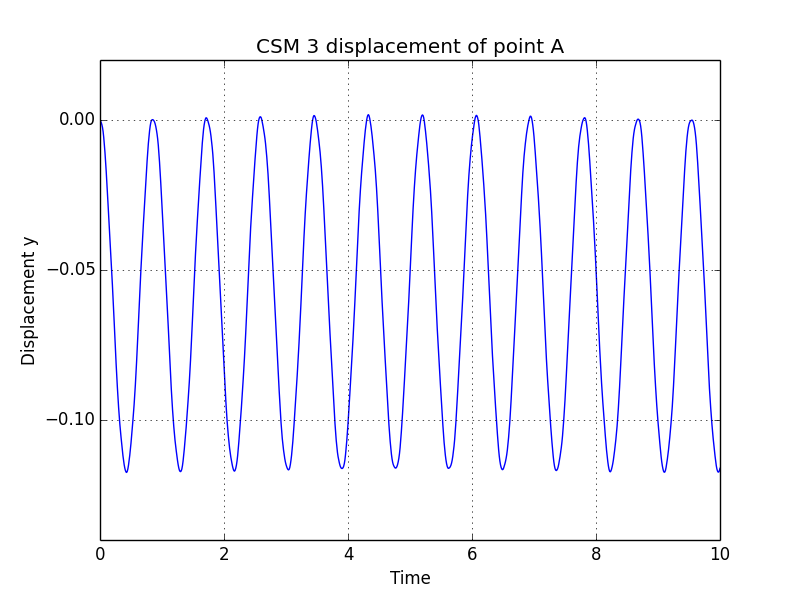
\includegraphics[scale=0.40]{./Temporal_stability/CSM3_Crank_y.png} 
    \caption{$\theta = 0.5 $} 
    \vspace{4ex}
  \end{minipage} 
 \label{fig:CSM3_dis_plots} 
 \caption {CSM3 displacements with $\Delta t = 0.01$ with different values for $\theta$}
\end{figure}


\subsubsection*{Discussion on numerical stability}
The shifted version of the Crank-Nicholson scheme is stable when computing for time step values as low as $\Delta t = 0.01$. However with $\Delta t = 0.001$ the normal Crank-Nicholson scheme ($\theta =0.5$) can be used and is long term stable. 
It has also been reported by Wick 2011 \cite{Wick2011} that the Crank-Nicholson, $\theta = 0.5$, scheme is stable throughout the computing time by setting $\Delta t = 0.001$.

In the FSI2 case the results for the finest mesh showed, in previous chapter, similar results for $\Delta t = 0.01$ and $\Delta t = 0.001$, meaning that the shifted version of the Crank-Nicholson scheme can be applied, in certain cases, with $\Delta t = 0.01$ greatly reducing computational runtime.

The CSM3 test shows that choosing $\theta = 0.5$ is crucial for preserving energy when computing solid problems.




